\documentclass{article}
\usepackage[utf8]{inputenc}
\usepackage[italian]{babel}
\usepackage{graphicx}
\usepackage{hyperref}
\usepackage{pgf-pie} % Pacchetto per grafici a torta
\usepackage{lscape} % Per pagine orizzontali
\usepackage{caption} % Per personalizzare le didascalie

\title{Deadline 1 – Needfinding}
\author{Mattia Colombo, Carmen Giaccotto, Alessia Franchetti-Rosada \\Federico Previtali, Manoueil Michael Halim Riad Hanna \\ Valentina Petrignano, Michele Arrigoni}
\date{14 Ottobre 2024}

\begin{document}

\maketitle

\section{Introduzione}

\subsection{Dominio di interesse e perché lo abbiamo scelto}

Siamo \textbf{DesignersForCulture}, un gruppo di ricerca nell'ambito della Human Computer Interaction presso il Politecnico di Milano, laureandi in Ingegneria Informatica. La nostra missione è esplorare e sviluppare soluzioni innovative che uniscano tecnologia e cultura, con l'obiettivo di rendere l'arte e il patrimonio culturale più accessibili e coinvolgenti.

Il nostro team è composto da studenti appassionati di tecnologia, design e cultura. Crediamo che l'integrazione di questi ambiti possa creare esperienze uniche che arricchiscono la società e promuovono la partecipazione attiva dei cittadini nel mondo dell'arte.

Attraverso progetti interdisciplinari, collaboriamo con musei, istituzioni culturali e scuole per progettare strumenti e applicazioni che facilitino l'interazione tra le persone e le opere d'arte. Il nostro obiettivo è non solo di innovare tecnicamente, ma anche di comprendere profondamente le esigenze degli utenti per creare soluzioni realmente efficaci e significative.

\section{Metodologia}

\subsection{Partecipanti}

I partecipanti selezionati per le interviste includono gestori di musei, insegnanti di liceo e adolescenti. Sono stati scelti per la loro esperienza diretta nel settore culturale e per rappresentare sia gli utenti lead che quelli non-lead. Gli adolescenti, in particolare, sono stati coinvolti per comprendere le loro esigenze e motivazioni riguardo alle esperienze museali. Gli utenti estremi comprendono persone che non frequentano i musei, al fine di identificare le barriere che impediscono la partecipazione culturale.

\subsection{Luogo delle Interviste}

Le interviste sono state condotte sia in presenza presso musei locali che online tramite piattaforme di videoconferenza, a seconda delle preferenze e disponibilità dei partecipanti.

\subsection{Organizzazione dell'Intervista}

Le interviste sono state organizzate in modo da esplorare diverse aree di interesse:

\begin{itemize}
    \item Per i \textbf{gestori museali} e gli \textbf{insegnanti di liceo}, le domande si sono focalizzate su come gli adolescenti interagiscono con l'arte, le sfide nel coinvolgerli e possibili strategie per aumentare il loro interesse.
    \item Per gli \textbf{adolescenti}, abbiamo esplorato le loro esperienze attuali con i musei, le preferenze, le barriere e le motivazioni che influenzano la loro partecipazione.
    \item Per le \textbf{persone che non frequentano i musei}, le domande miravano a comprendere le ragioni del loro disinteresse e a raccogliere suggerimenti su come rendere i musei più attraenti.
\end{itemize}

\subsection{Ruolo dei Membri del Gruppo}

Mattia Colombo ha svolto il ruolo di intervistatore principale, conducendo le interviste e raccogliendo i dati. Ha anche coordinato la comunicazione con i partecipanti e ha curato la trascrizione delle interviste.

\subsection{Materiale Usato}

Durante le interviste sono stati utilizzati:

\begin{itemize}
    \item Registratore audio (previo consenso dei partecipanti) per garantire l'accuratezza dei dati raccolti.
    \item Notebook per prendere appunti durante le interviste.
    \item Software di videoconferenza per le interviste online.
\end{itemize}

\section{Risultati delle Interviste}

\subsection{Fotografie e Artefatti Rilevanti}

\begin{figure}[h]
\centering
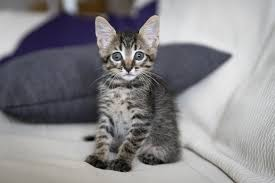
\includegraphics[width=0.5\textwidth]{p1.jpg}
\caption{Esempio di materiale promozionale del museo condiviso durante l'intervista.}
\end{figure}

\subsection{Citazioni Chiave Rilasciate dagli Utenti}

\begin{itemize}
    \item \textbf{Gestore museale}: "Gli adolescenti spesso trovano i musei poco coinvolgenti; dobbiamo innovare le modalità di interazione."
    \item \textbf{Insegnante di liceo}: "Integrando la tecnologia nelle visite, potremmo stimolare maggior interesse nei ragazzi."
    \item \textbf{Adolescente}: "Mi piacerebbe se i musei fossero più interattivi, magari con giochi o sfide."
    \item \textbf{Non frequentatore di musei}: "Non vado al museo perché lo trovo noioso e non mi sento coinvolto."
\end{itemize}

\section{Risultati del Survey}

Abbiamo distribuito un sondaggio per raccogliere dati preliminari sugli utenti, in particolare adolescenti e giovani adulti. I risultati ci hanno fornito un quadro utile delle loro esperienze con i musei e delle loro aspettative.

\subsection{Link al questionario}

Il questionario completo può essere consultato al seguente link: \url{https://bit.ly/4eu3ox7}

\subsection{Demografia dei Partecipanti}

Il sondaggio ha coinvolto principalmente partecipanti di età compresa tra i 16-19 anni e oltre i 20 anni, con una rappresentanza femminile predominante. La maggior parte dei partecipanti risiede in piccole città o paesi, sebbene ci siano stati anche rispondenti provenienti da aree urbane.

\subsection{Frequenza di Visita ai Musei}

Quando è stato chiesto quante volte avevano visitato un museo negli ultimi 12 mesi, la maggior parte dei partecipanti ha indicato tra le 3 e le 5 visite, con alcuni che hanno dichiarato di aver visitato musei più di 5 volte.

\subsection{Suggerimenti per il Miglioramento dell'Esperienza Museale}

Diversi partecipanti hanno offerto suggerimenti per migliorare l'esperienza museale. Ad esempio, un partecipante ha proposto di "perfezionare e dettagliare i percorsi tematici per renderli più coinvolgenti", mentre altri non hanno riscontrato aree di miglioramento. Alcuni commenti indicano un certo livello di soddisfazione generale, ma c'è ancora spazio per aumentare il coinvolgimento.

\subsection{Disponibilità a Partecipare a Ulteriori Interviste}

Abbiamo anche chiesto ai partecipanti se fossero disposti a rispondere a ulteriori domande o a partecipare a interviste individuali. La maggior parte ha preferito non essere contattata, anche se alcuni hanno lasciato i loro contatti per un coinvolgimento futuro.

\section{Logica del form}

\vspace*{\fill}
\begin{center}
    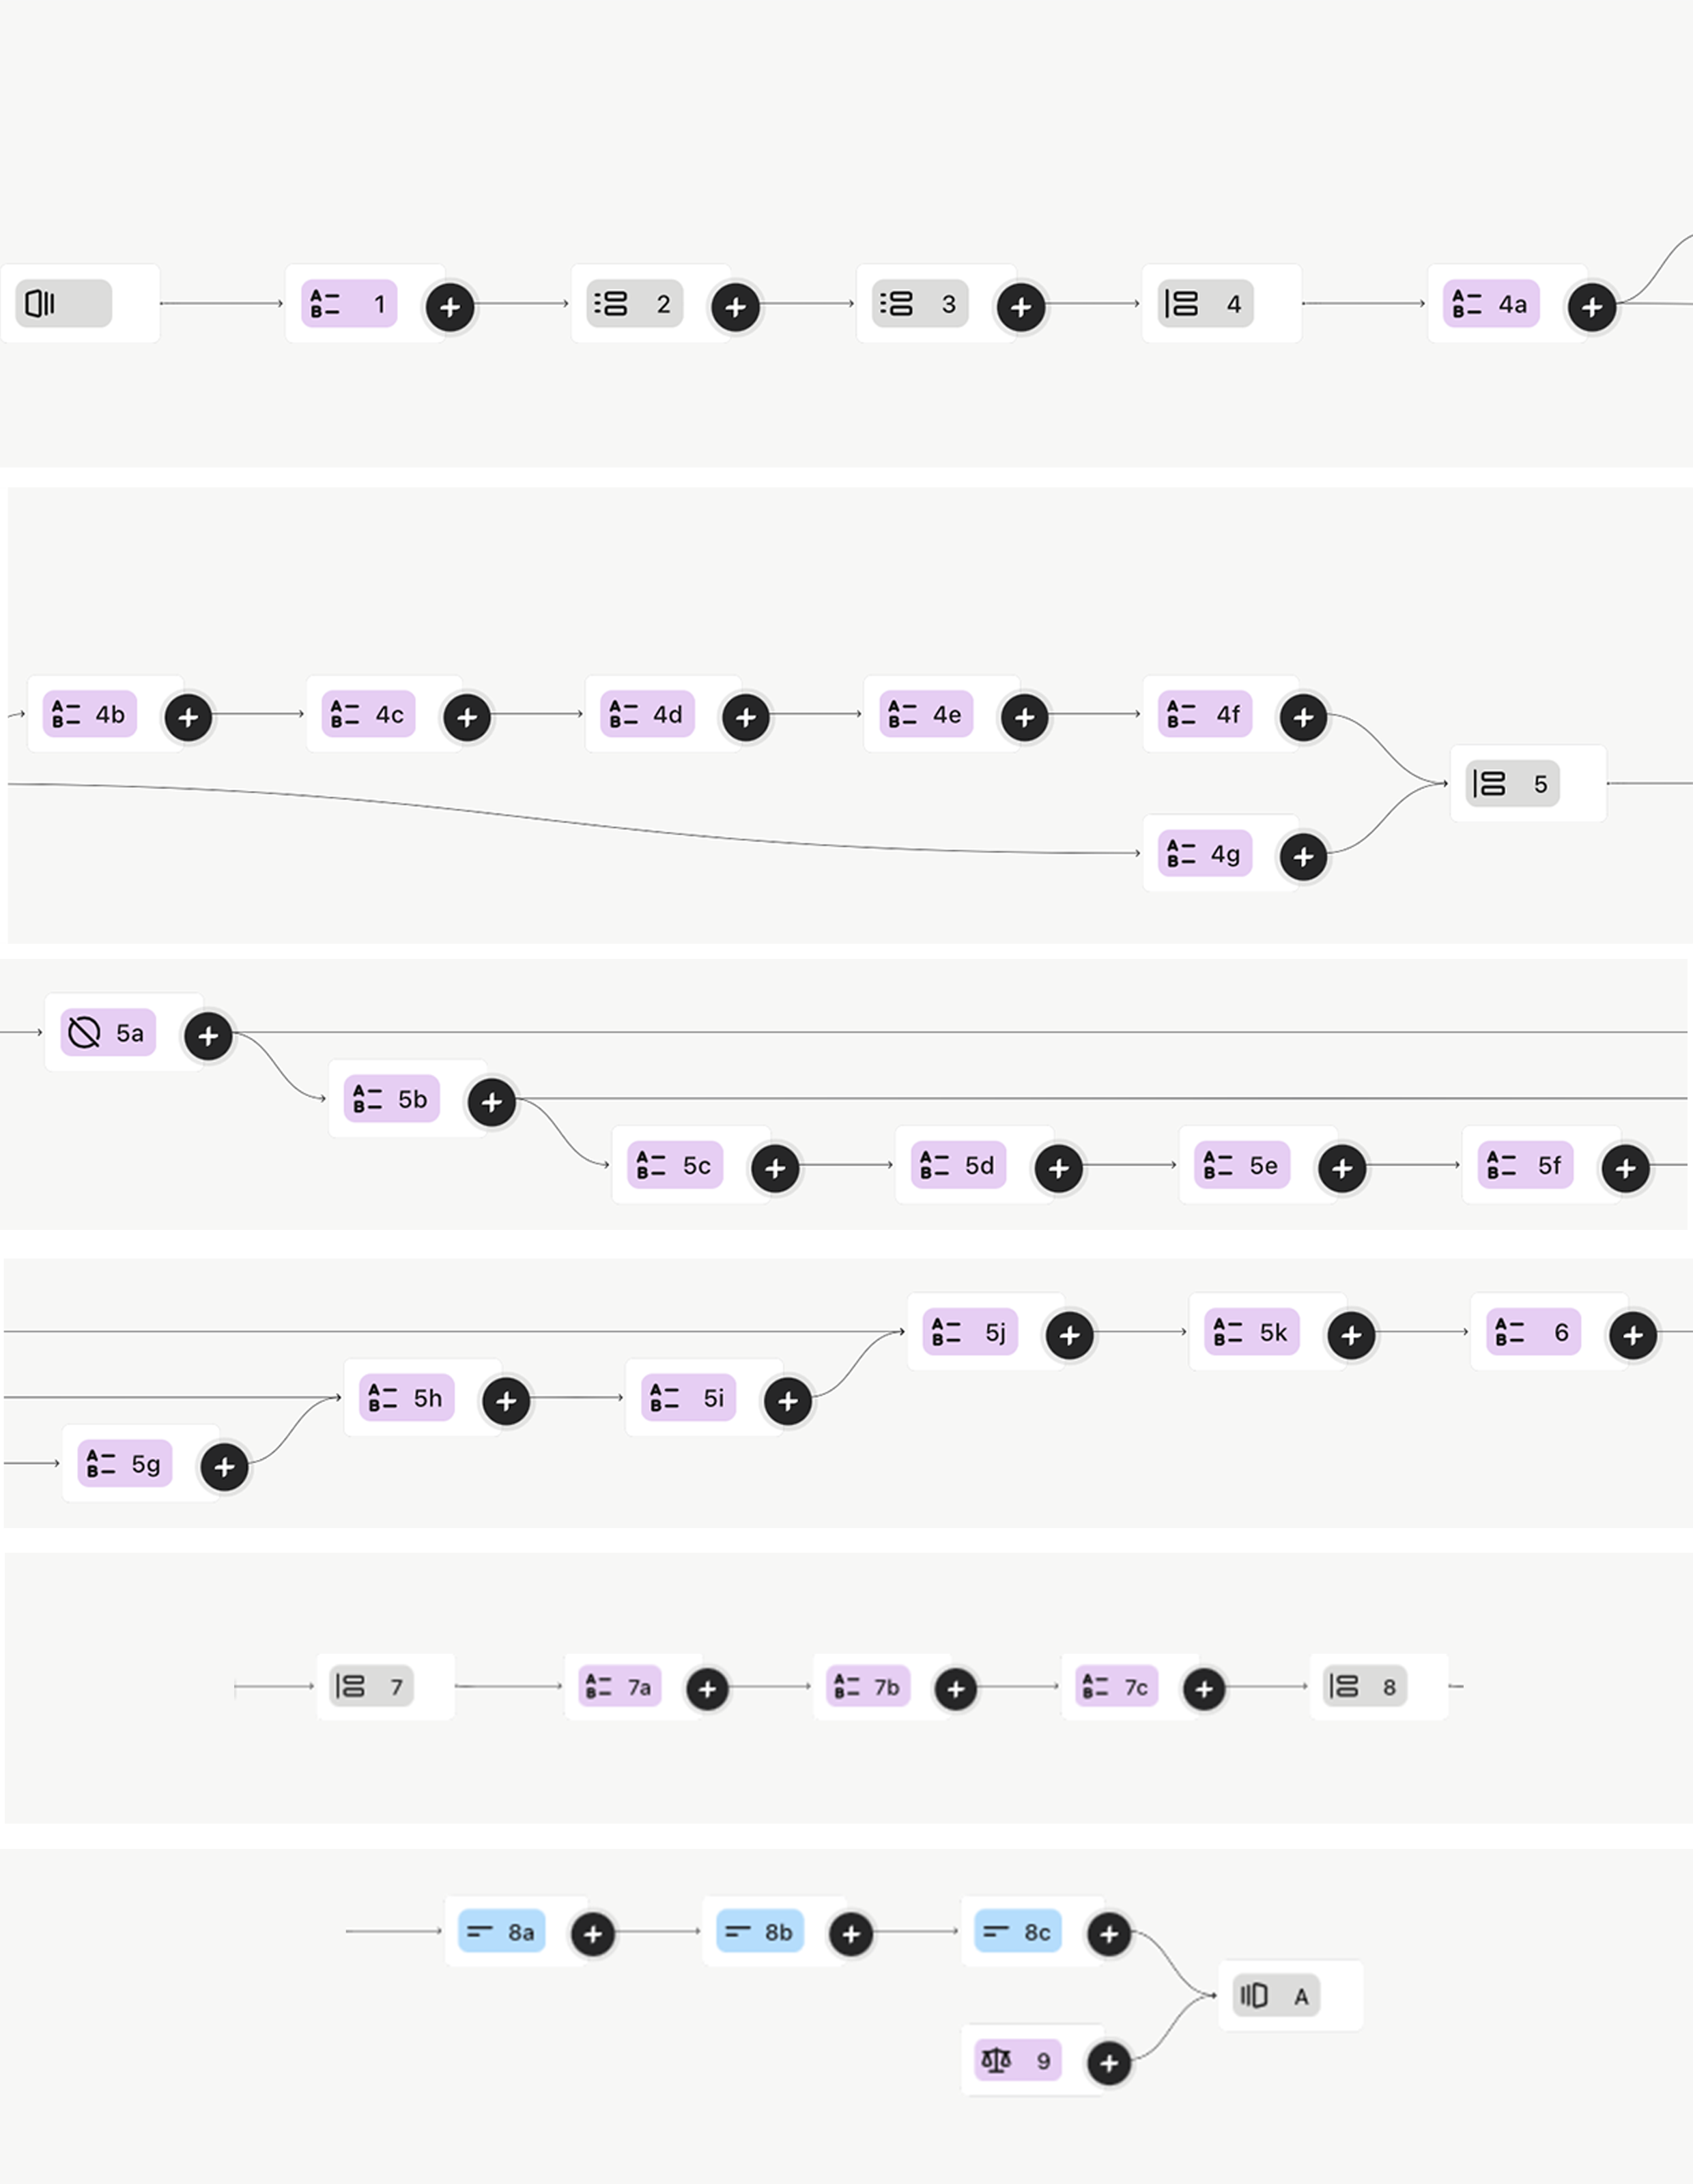
\includegraphics[width=\textwidth]{form_logic.png} % Immagine della logica del form (da inserire)
\end{center}
\vspace*{\fill}
\newpage

\section{Foto Affinity Diagram Esercitazione}

\vspace*{\fill}
\begin{center}
    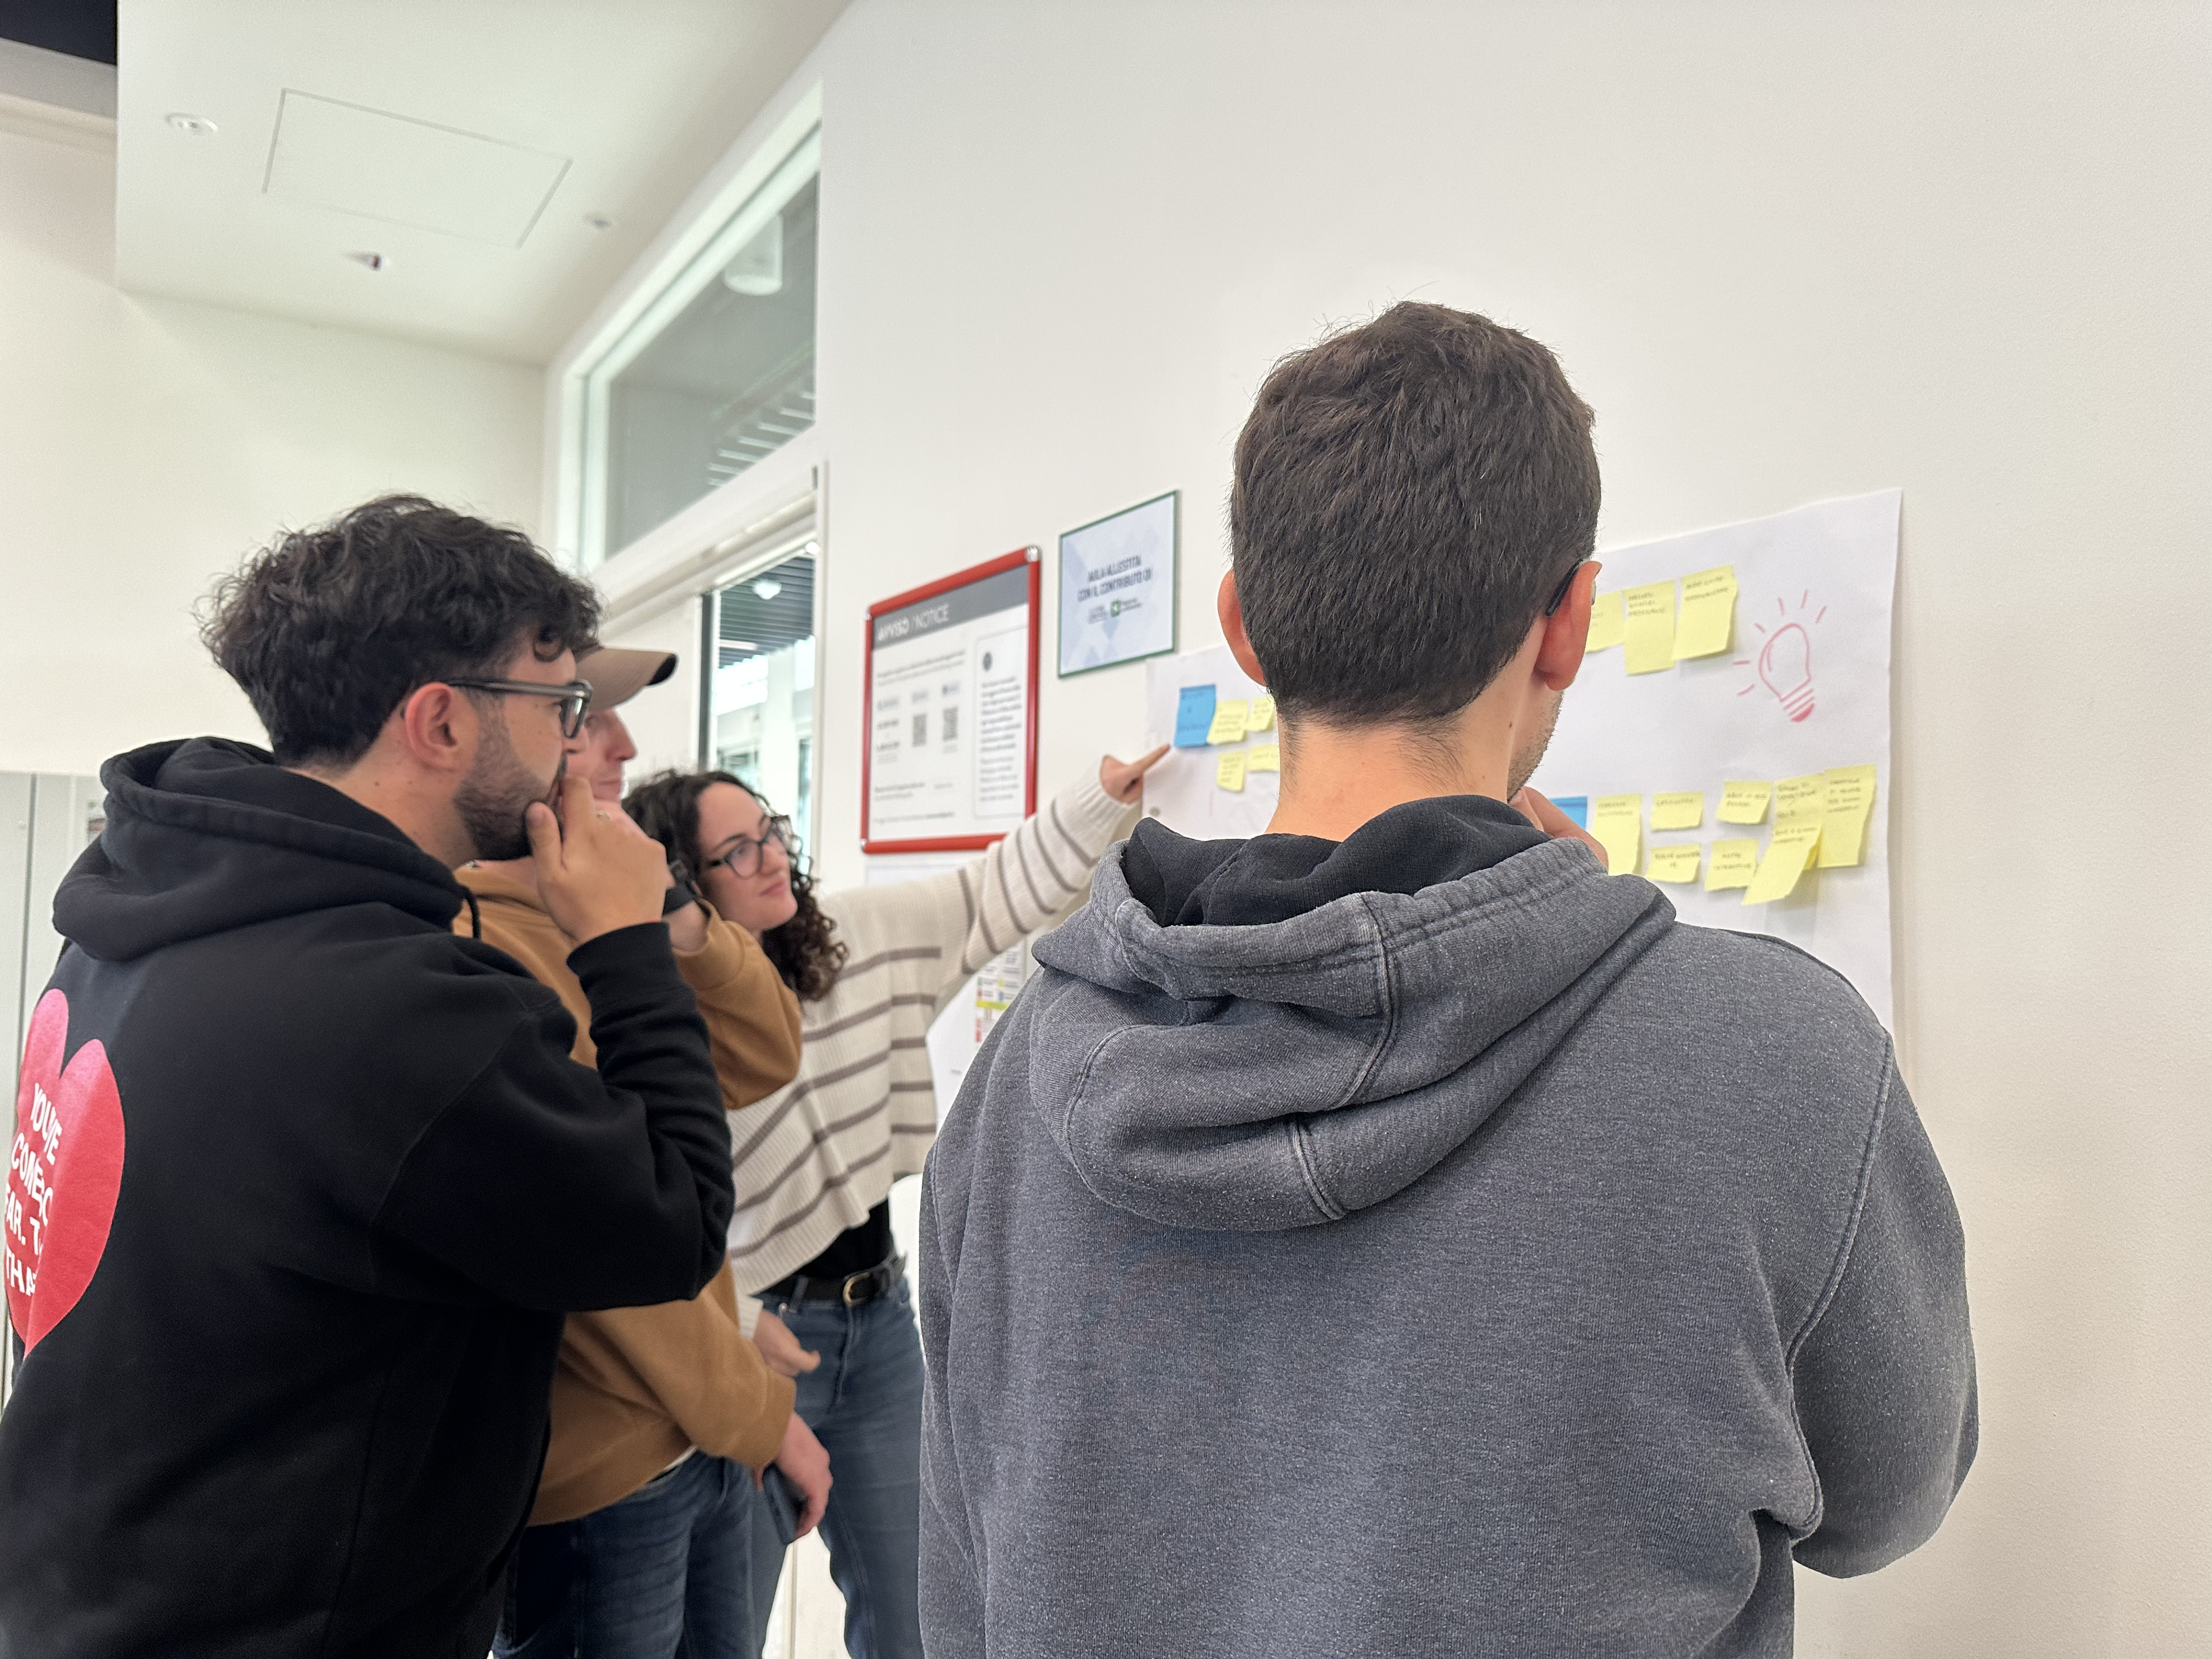
\includegraphics[width=\textwidth]{affinity_diagram.png} % Spazio per foto Affinity Diagram
\end{center}
\vspace*{\fill}
\newpage

\section{Grafici a Torta per i Dati del Survey}

\begin{figure}[h]
    \centering
    \begin{tikzpicture}
        \pie[text=legend, radius=3, color={red!30, blue!30, green!30, yellow!30}]{
            40/16-19 anni,
            35/20-25 anni,
            25/Oltre 25 anni
        }
    \end{tikzpicture}
    \caption{Distribuzione dell'età dei partecipanti.}
\end{figure}

\begin{figure}[h]
    \centering
    \begin{tikzpicture}
        \pie[text=legend, radius=3, color={red!50, blue!50}]{
            60/3-5 visite,
            40/Più di 5 visite
        }
    \end{tikzpicture}
    \caption{Frequenza di visita ai musei negli ultimi 12 mesi.}
\end{figure}
\newpage

\section{Sintesi}

\subsection{Mappa Iniziale tra Utenti e Obiettivi}

\begin{itemize}
    \item \textbf{Adolescenti} $\rightarrow$ Ricerca di interattività e coinvolgimento attraverso la tecnologia e gamification.
    \item \textbf{Gestori museali} $\rightarrow$ Necessità di strumenti innovativi per attirare un pubblico più giovane.
    \item \textbf{Insegnanti} $\rightarrow$ Interesse a integrare esperienze museali nel contesto educativo.
    \item \textbf{Non frequentatori} $\rightarrow$ Riduzione delle barriere percepite e aumento della rilevanza personale delle offerte museali.
\end{itemize}

\subsection{Bisogni degli Utenti più Significativi}

\begin{itemize}
    \item Creare esperienze museali più interattive e coinvolgenti per gli adolescenti.
    \item Facilitare l'accesso a informazioni e audioguide tramite dispositivi personali.
    \item Integrare elementi di gioco e competizione per aumentare l'interesse.
    \item Migliorare la comunicazione e la promozione delle attività museali attraverso canali digitali.
\end{itemize}

\section{Passi Futuri}

\begin{itemize}
    \item Analizzare in dettaglio i dati raccolti per identificare requisiti specifici.
    \item Sviluppare prototipi di soluzioni tecnologiche basate sui bisogni emersi.
    \item Condurre test di usabilità con utenti rappresentativi per valutare le soluzioni proposte.
    \item Collaborare con musei e istituzioni per implementare e affinare le soluzioni.
\end{itemize}

\end{document}